\Lecture{Jayalal Sharma}{Sept 19, 2020}{08}{Live lecture discussion}{Anshu and Narasimha Sai }{$\alpha$}{JS}

\paragraph{Bijection from Euler's problem to Binary Trees} As we have already established a bijection from set of balanced parenthesisations to set of full binary trees and established that number of full binary trees with $n$ internal nodes is the catlan number $C_n$, in this section, let's establish a bijection from the \emph{Euler's Problem} to set of full binary trees to establish that the solution to \emph{Euler's problem} is also catlan number $C_n$.

Lets recall \emph{Euler's problem} first. Consider a convex polygon with $n+2$ edges. Euler's problem is the number of ways of triangulating it (partition the polygon into triangles) by drawing non-crossing diagonals. (Refer fig. \ref{fig:Euler's-polygon}). We know that number of non-crossing diagonals in a polygon of $n+2$ edges is $n-1$ (proof follows from a simple induction) and from those $n-1$ non-crossing diagonals, we have our polygon partitioned into $n$ triangles. Let's associate each of the triangles with a vertex (green dots in the fig. \ref{fig:Euler's-polygon}). Observe that if two triangles share an edge, it must be one of the diagonals (no two triangles can share an edge because of non-crossing diagonals). Now, let's connect the vertices whose corresponding triangles share an edge. Any edge connecting two of these vertices crosses a diagonal. 
\begin{figure}[h!]
    \centering
    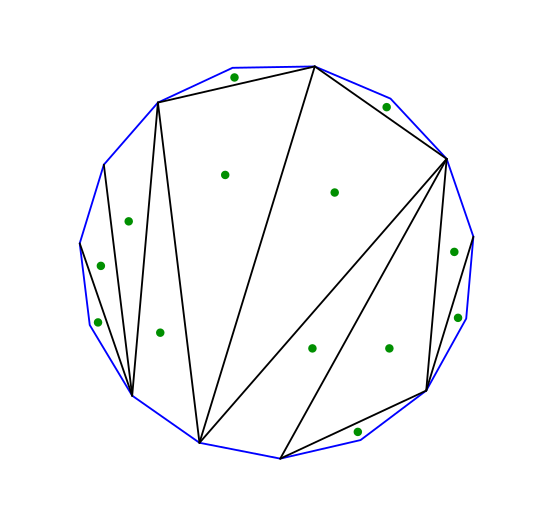
\includegraphics[width=0.4\linewidth]{polygon.png}
    \caption{Partitioning a polygon into triangles by non-crossing diagonals. Observe that green dots in each triangle associates the triangle with a vertex}
    \label{fig:Euler's-polygon}
\end{figure}
Now, consider a polygon edge $e$. For every polygon edge surrounding a vertex (other than $e$), add an open-edge originating from that vertex (see fig. \ref{fig:tree-in-polygon}). We arrive at the following claim.  
\begin{claim}
	If we remove the underlying triangles (which are formed with polygon edges and diagonals), from fig. \ref{fig:tree-in-polygon}, the 		resulting graph obtained (see fig. \ref{fig:tree}) is a full binary tree with the vertices as internal nodes.
\end{claim}
\begin{figure}[h!]
    \centering
    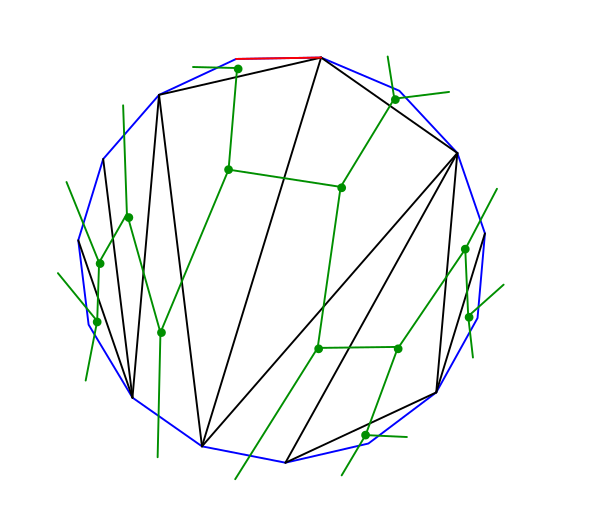
\includegraphics[width=0.4\linewidth]{polygon-tree.png}
    \caption{Polygon with vertices connected to form a tree}
    \label{fig:tree-in-polygon}
\end{figure}
\begin{figure}[h!]
    \centering
    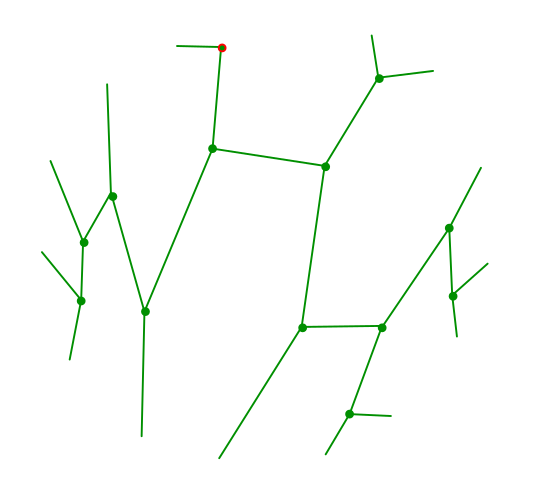
\includegraphics[width=0.4\linewidth]{tree.png}
    \caption{Tree formed by connecting vertices}
    \label{fig:tree}
\end{figure}
\begin{proof}
	We observe that degree of every vertex other than the vertex surrounded by edge $e$ is 2. This vertex will act as root to our full binary tree. All other vertices have degree 3 because each vertex is surrounded by a triangle and if a side is a diagonal, it will be connected to vertex which is surrounded by triangle that shares the diagonal and if the side is a polygon edge, then there will be an open edge corresponding to it originating from the vertex. Therefore the resulting graph formed is a full binary tree with our vertices as $n$ internal nodes and vertices corresponding to open edges are $n+1$ leaves (because there are $n+2$ edges and one edge is under consideration). This completes the description of bijection.
\end{proof}

We leave it as an exercise to the reader to prove that the mapping defined above is indeed a bijection.

\paragraph{Bijection from binary trees to full binary trees}
In this section we are interested in connection between binary and full binary trees. Recall that a full binary tree is one in which each node has either 0 or two children. On the other hand, when we say binary tree then it only means that each node can have at most two children. We want to find a bijection between set of binary trees with $n$ internal nodes and set of full binary trees with certain number of internal nodes. 

First of all lets try to see how to convert a given binary tree into a full binary tree so that we can reverse the process, i.e. recover the original (binary) tree back from the full binary tree without ambiguity. 

Here is the first attempt:

\noindent \underline{Attempt 1:} First natural approach can be to add a leaf node to all non-full (internal nodes having only one child) nodes, as shown in figure~\ref{fig:bt-fbt-attempt1}
\begin{figure}[h!]
    \centering
    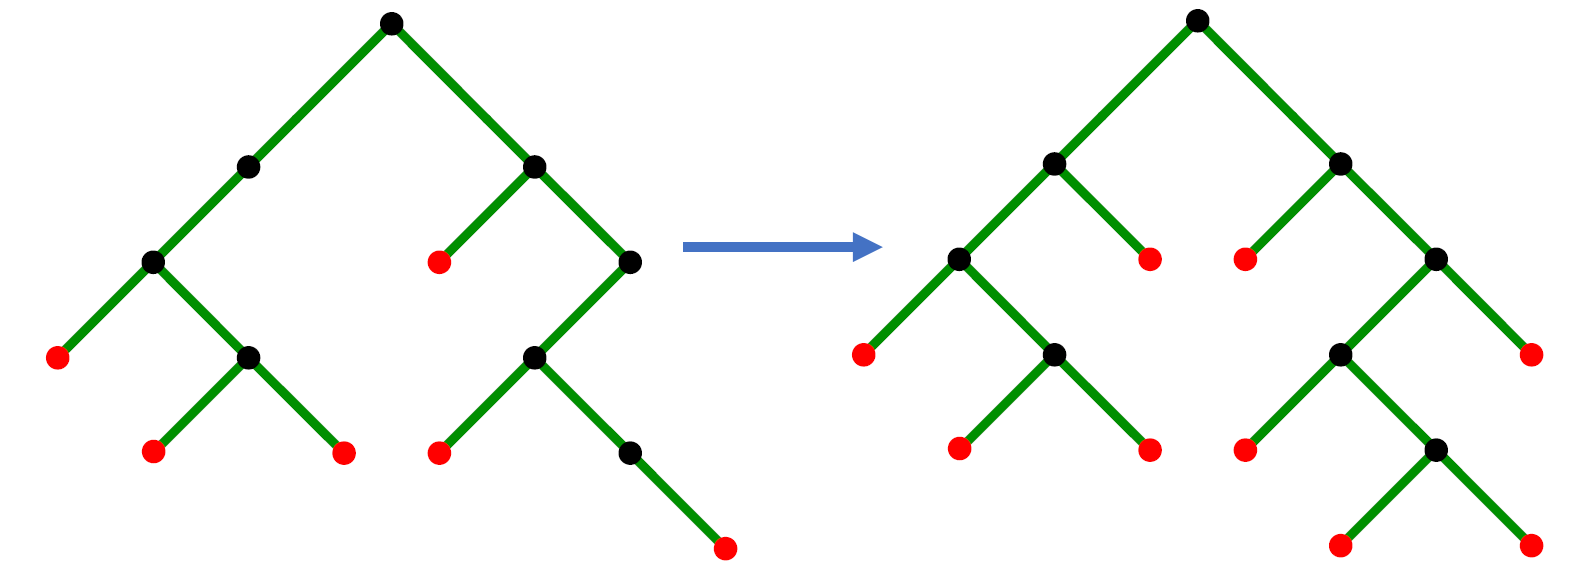
\includegraphics[width=0.7\linewidth]{binary-to-full-binary-1.png}
    \caption{Binary to full binary tree attempt1: adding a child node to each non full node}
    \label{fig:bt-fbt-attempt1}
\end{figure}

But notice that this transformation is not injective. For example, it can be observed that  both the trees in figure~\ref{fig:bt-fbt-attempt1-issue} map to same full binary tree.
\begin{figure}[h!]
    \centering
    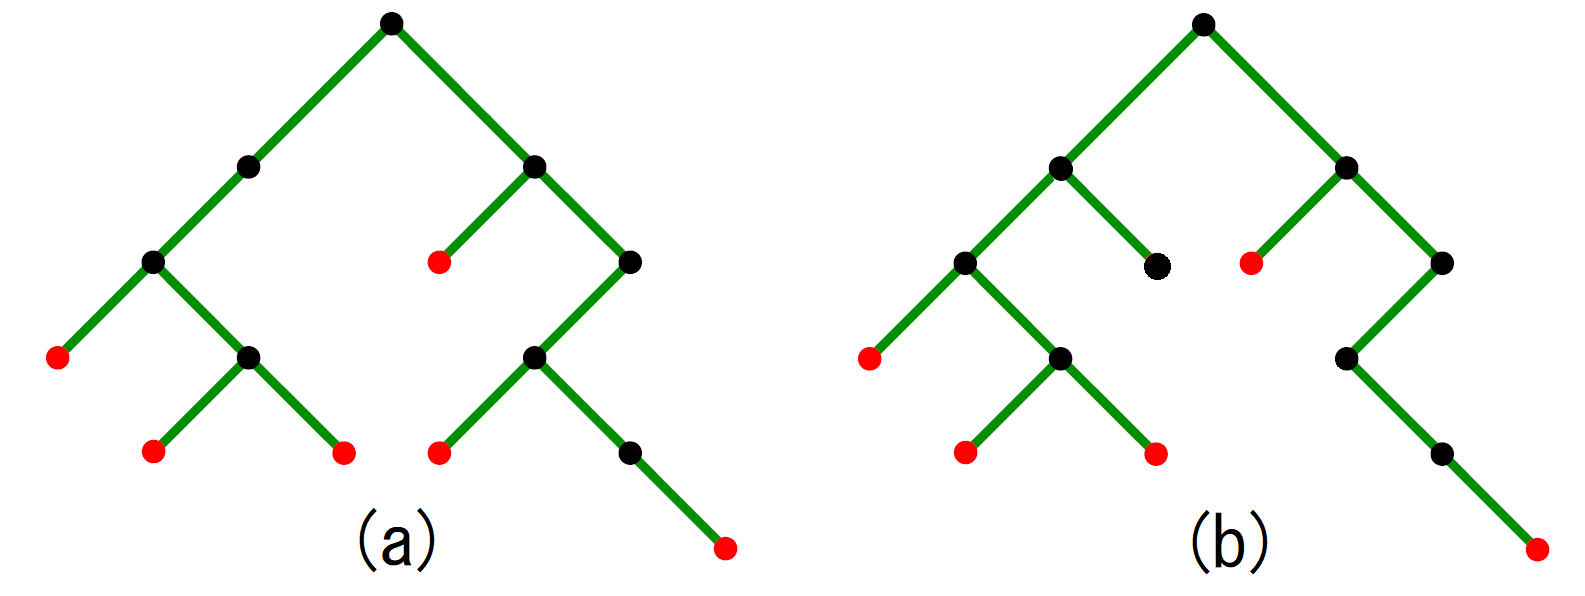
\includegraphics[width=0.7\linewidth]{binary-to-full-binary-2.png}
    \caption{Two different binary trees that map to same full binary tree}
    \label{fig:bt-fbt-attempt1-issue}
\end{figure}

\noindent\underline{Attempt 2(correct)}
Lets try a slightly different approach. Given a binary tree, do the following:
\begin{itemize}
    \item to each leaf node, add two children
    \item to each internal node having only one child, add another child
\end{itemize}
Figure~\ref{fig:binary-to-full-solution} shows the full binary tree constructed in this way for the same binary tree as in Figure~\ref{fig:bt-fbt-attempt1}.
\begin{figure}[h!]
    \centering
    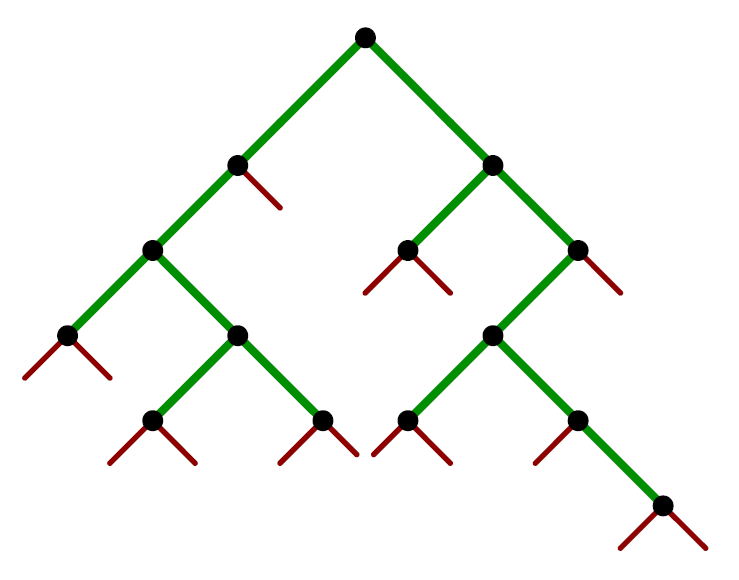
\includegraphics[width=0.5\linewidth]{full-binary-3.png}
    \caption{Full binary tree for the (non-full) binary tree given in fig~\ref{fig:bt-fbt-attempt1}. Notice that all the leaf nodes are added during transformation}
    \label{fig:binary-to-full-solution}
\end{figure}
We can see that this solution addresses the issue in the first attempt. Intuitively because of following argument: in the previous attempt the problem was that given a full binary tree, it was hard to decide if a leaf node was originally present in the binary tree or added during transformation. Now, in the current solution, this issue does not arise, because for any leaf node originally present in the binary tree, we add two new leaves as its children. Thus, it can be observed that all the leaf nodes (and only these nodes) are added during transformation.

To see that this translation is well-defined, we can see that the transformed tree is full binary tree by construction itself. Surjectivity is also easy to prove. To recover a binary tree from any given full binary tree, simply remove all the leaf nodes. We discussed injection informally. To give a formal argument, we first need to identify how to characterize two different binary trees? One of the hint as given during the discussion is to assign address to the nodes in the form of binary string, where 0-1 represents left or right child. 

Here we argued the bijection only intuitively and there are many things to be worked out formally. For example, proof for injection is not formally argued. Also, to argue surjection, we need to fix the number of nodes in full binary tree. Once we figure out this number, the argument for transformation being  well-defined also need to take that into account.

Writing a complete formal proof of bijection is left as homework exercise.

\paragraph{Bijection between plane trees and full binary trees}
A plane tree is a rooted tree with an ordering among the children. A plane tree can have more than two children. Figure~\ref{fig:plane-tree-1} shows a plane tree. 

\begin{figure}[h!]
    \centering
    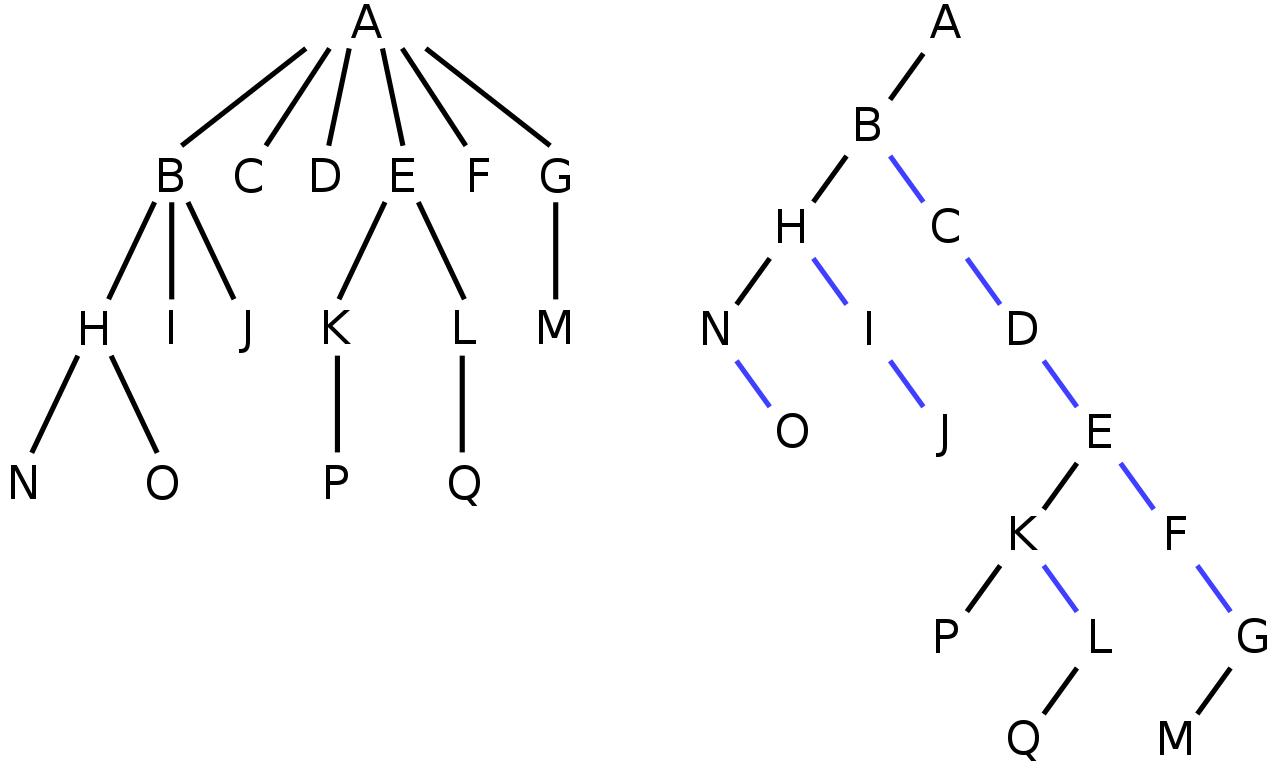
\includegraphics[width=0.8\linewidth]{plane-tree.png}
    \caption{An example of plane trees and its transformation to a binary tree}
    \label{fig:plane-tree-1}
\end{figure}

We are interested in studying the connection between plane trees and binary trees. The number of plane trees with $n$ nodes is equal to the number of binary trees with $n$ nodes. Thus, there is bijection between set of plane trees with $n$ nodes and the set of  binary trees with $n$ nodes. 

Here we define the bijection function. 

\noindent\underline{The Bijection:} Given any plane tree, do the following
\begin{itemize}
    \item For each node in the tree, 
    \begin{itemize}
        \item add its first child in plane tree as its left child in binary tree
        \item add its immediate sibling on right as its right child in binary tree.
    \end{itemize} child in the binary tree.
\end{itemize}
By following the above rule, we get a binary tree from given plane tree.

Observe that in the binary tree thus obtained, root node has only one child, while in general, in a binary tree the root can have both its children. Hence, we won't include the root as part of the binary tree.

Writing formal argument for all the properties is left as homework excercise.
